\documentclass[conference]{IEEEtran}
\IEEEoverridecommandlockouts

\usepackage{cite}
\usepackage{amsmath,amssymb,amsfonts}
\usepackage{graphicx}
\usepackage{textcomp}
\usepackage{xcolor}
\usepackage{booktabs}
\usepackage{array}
\usepackage{algorithm}
\usepackage{algpseudocode}
\usepackage{dblfloatfix}
\usepackage{float}

\graphicspath{{images/}}

\begin{document}

\title{Analysis of Minimax Adversarial Search Optimizations in Connect 4}

\author{
    \IEEEauthorblockN{Jacob A. Geldbach}
    \IEEEauthorblockA{
        \textit{College of Engineering: CS} \\
        \textit{University of Idaho} \\
        Moscow Idaho, United States \\
        geld8788@vandals.uidaho.edu
    }
}

\maketitle

\begin{abstract}
    Adversarial search is a topic of search related to zero-sum scenarios between two opponents with directly opposing goals. The goal of this project was to implement and analyze the Minimax algorithm in the context of a game of Connect 4. The Minimax implementation is used for the AI player to generate the best possible move it can make given the current board state. In the scenario of an AI player vs an AI player both players utilized the exact same Minimax implementation to find the next best move. This implementation allows for Connect 4 to be played with an AI opponent of varying difficulty where difficulty is set by the number of turns the AI player is allowed to look ahead in the Connect 4 Minimax built game tree. The project includes multiple different adversarial search algortihm optimizations that are able to be included or excluded from a specific run of the program, allowing for comparison of the collected analytical data. Alpha-beta Pruning, Iterative Deepening combined with Move Re-ordering and Selective Deepening (Quiescent Search) were all used on top of the base Minimax algorithm to further improve its efficiency in regards to time per turn and nodes explored.

\end{abstract}

\begin{IEEEkeywords}
    Adversarial, Search, Minimax, Connect4, Efficiency, Alpha, Beta, Pruning, Quiescent

\end{IEEEkeywords}

% -------------------------------------------------------

\section{Algorithm}
Minimax is an algorithm based on mutually recursive calls to a minMove and a maxMove function. Each layer of the recursive calls is effectively the AI looking one more turn ahead. And due to the adversarial environment that this algorithm is built for, each layer is finding either the best move for that player or the worse move for that player given the current board state. The board state is also evolving as the algorithm works down to the max depth for the call, as each layer is calling the min/maxMove() function for each of the possible valid moves at that layer. When the recursive calls hit the max depth that Minimax was called with, an evaluation of the board with that path of prospective moves is returned up the tree. This evaluation is a heuristic, as if the algorithm has reached this far in the search an estimation of how good or bad this board state is for the player must be returned. The evaluation function I used in this project is defined below in more detail. Each layer of the recursion all final states of the board are checked such as a win for the player, a loss for the player or the board has filled up entirely and it is to end in a draw. When these states are found the extremes of the board value spectrum (-inf, inf) are returned to influence the Minimax towards or away from them (win or lose). Once each mutually recursive call of min/maxMove pertaining to one of the current valid possible moves returns in the root Minimax function, each value is compared and the move corresponding with the highest value is returned and officially played by the AI for that turn. The time efficiency of this Minimax implementation is $O(b^d)$ nodes processed per turn of the AI, where $b$ is number of valid moves or columns and $d$ is depth of tree look ahead or turns the AI can look ahead and. The space efficiency is much better at $O(b*d)$ since only the exact path down to the current node or the current recusion stack of nodes is kept in memory at a single time.

\subsection{Evaluation Function}
The evaluation function used in this project was a tally of the entire boards "score". Where each indivual window, defined as 4 spaces in a row vertically, horizontally and diagnoally, is scored based on how "good" or likely a player is to win or lose with that number of their pieces in a single window. There are a total of 69 total scorable windows, leading this evaluation function to be space and time O(1) efficient. Most importantly the score for a single window is significantly better for each consectutive piece a player has in a non-contested window. So for example a single piece in a non-contested windown (meaning only their pieces and empty slots make up the window) is good, but two of their pieces is scored quadratically more opposed to just 2 times the window with 1 piece. As soon as a window becomes contested it is worth 0 points towards the total evaluation of that board as there is no way to win or lose via that window. Non-contested windows with 3 of a players pieces are valued far more than 2 piece windows because that window is also a win condition on the next turn. All of these scores are the negated values for when it is the opponents pieces instead of the players pieces. With the exception that opponent 3 piece windows are negatively valued even more than the 3 piece windows of the player resulting in the AI player prioritizing the blocking of potential winning moves for their opponent so they do not lose the game.

\subsection{Alpha--Beta Pruning}
Alpha-Beta Pruning is an optimization technique that was used in this project's implementation. Alpha-Beta Pruning allows for upper and lower bounds to be passed down to each layer of the mutually recursive calls of min/maxMove. What this allows for is in maxMove the lower bound can be checked against the prospective value being returned by each call to minMove, if the value returned from minMove is greater than the current lower bound, that call of maxMove knows it will never pick anything less than that value so it updates the lower bound to reflect that. The same is done in minMove except the inverse and with the upper bound. As these bounds converge or tighten this informs the different layers that as soon as a call of minMove sees the upper bound go lower or equal to the lower bound the program can return from that call and essentially prune all remaining (6 down to 1) child nodes for that branch. The reason for this is that minMove knows that the maximizer somewhere along the way higher up in the tree has at worst the lower bound. The alpha and beta values are passed down per call to minMove and maxMove so that alpha lower bound value is inherited from a parent call to maxMove. The same but inverse is true about maxMove and its relationship with the beta upper bound, it knows that somewhere up above in the tree a minimizer layer has at worst the beta upper bound value meaning it can prune all of that move nodes child branches once it sees the alpha lower bound value become equal to or greater than the beta upper bound value. It is important to note that Alpha-Beta pruning is only an optimization in regards to number of node processing efficiency, meaning it will not alter the algorithm to where it will now start making different decisions regarding what move to make. Minimax will make the same move choice as it would have without using Alpha-Beta pruning except it potentially can make the same choice in a fraction of total nodes processed. Alpha-Beta pruning on average takes Minimax from a time efficiency $O(b^d)$ to $O(b^{3d/4})$. Wherein combined with some of the techniques expanded on in below sections it can reach time efficiencies of $O(b^{d/2})$.

\subsection{Iterative Deepening and Move Re-Ordering}
Move Re-Ordering and Iterative Deepening are two more time efficiency optimization techniques used in this project's implementation. These optimizations are used in conjunction with Alpha-Beta pruning in order to accelerate the rate at which branches are pruned early in the search of the game tree by Minimax. The true optimization that is occurring comes from the order in which the move branches of a node are explored. By exploring the higher valued moves first (moves that lead to a higher valued board evaluation), this leads to the Alpha-Beta pruning ranges being tightened earlier in the search, and with a tighter upper and lower bound range, more branches and entire subtrees of the game tree will be pruned off. Move Re-Ordering in this project is used even in the default run of the algorithm. The algorithm is sorting the list of valid column moves by center, or instead of iterating over the possible moves starting at column 0 to column 6, it looks at the central columns first. The reason for this is that it is well known that center pieces make up winning windows much more often than end column piece positions. This Move Re-Ordering alone led to fewer nodes needing to be processed per AI turn. The real efficiency improvement related to Move Re-Ordering came from its pairing with Iterative Deepening. What this allowed was for a dynamic best order of which moves to explore at the root of the Minimax search. The way this works is instead of following the same static center sorted order of move exploration for the entire $d$ depth Minimax search, the most "interesting" move ordering is calculated after each iterative call to Minimax. The way it was implemented in this project is Minimax with Alpha-Beta pruning and a depth of 1 is run using the center sorted order of move exploration, once that returns, it doesn't just return the best move at that depth; it returns a ranking list of the best moves. Then another Minimax search is called at depth 2 using the new best move ranked order for the order in which it explores the root's moves. And this is repeated until the max depth for the parent call to Minimax is hit.

\subsection{Selective Deepening (Quiescent Search)}
The final optimization that was included in this project is Selective Deepening. This is a adverserial search technique that allows for threat states to be marked, and allow that specific search path through the tree to continue another layer past the current max depth limit. In this implementation of Minimax when a game tree search path gets to the max depth and the evaluation function flags that board state as a possible threat, such as a non-contested window already holding three of one color, meaning a win or loss is available on the very next move. Selective Deepening would then allow the search to instead extend its search one layer deeper to further explore that threat and to more importantly thwart any game ending scenarios just beyond the horizon. Thereform  the impending win or loss is resolved as a true terminal value of -inf rather than returned up the tree as a heavier weighted negative value. This threat flag is produced by the same window scan the evaluation function already performs, so identifying the threat adds no extra pass over the board. But to be clear this implementation of Selective Deepening does not continue to go further on until the path is "quiet" or non-threat anymore. It simply extends a single layer of depth to protect the AI player from the Horizon Effect. Unlike the previous optimizations Sellective Deepening can change the move the AI ultimately plays: by looking one move beyond the horizon it can secure a win or block a loss that a strict fixed-depth search would have evaluated as merely a strong or weak position. 

% -------------------------------------------------------

\onecolumn
\section{Analysis}

\begin{table}[H]
\caption{Connect 4 --- Algorithm Analytics}
\begin{center}
\footnotesize
\setlength{\tabcolsep}{6pt}
\begin{tabular}{c >{\centering\arraybackslash}p{0.95in} >{\centering\arraybackslash}p{1.0in} >{\centering\arraybackslash}p{0.7in} >{\raggedright\arraybackslash}p{1.5in}}
\toprule
\textbf{Depth} & \textbf{\shortstack{Total States\\Explored}} & \textbf{\shortstack{First Move\\Explored States}} & \textbf{\shortstack{Time/\\Move}} & \textbf{Outcome} \\
\midrule
\multicolumn{5}{l}{\textbf{Minimax}} \\
4 & 25519 & 2800 & 0.502s & Blue win after 32 turns \\
5 & 150015 & 19607 & 0.958s & Blue win after 32 turns \\
6 & 839984 & 137256 & 2.985s & Blue win after 38 turns \\
\midrule
\multicolumn{5}{l}{\textbf{Minimax + Alpha--Beta}} \\
4 & 7286 & 857 & 0.430s & Blue win after 32 turns \\
5 & 36661 & 3282 & 0.513s & Blue win after 32 turns \\
6 & 43007 & 14552 & 0.625s & Blue win after 38 turns \\
\midrule
\multicolumn{5}{l}{\textbf{Minimax + Alpha--Beta + Static Move Re-Ordering}} \\
4 & 5921 & 188 & 0.430s & Blue win after 34 turns \\
5 & 25189 & 1091 & 0.499s & Red win after 27 turns \\
6 & 43007 & 1690 & 0.547s & Red win after 33 turns \\
\midrule
\multicolumn{5}{l}{\textbf{Minimax + Alpha--Beta + Move Re-Ordering and Iterative Deepening}} \\
4 & 6721 & 310 & 0.425s & Blue win after 36 turns \\
5 & 29783 & 1449 & 0.476s & Draw after 42 turns \\
6 & 59725 & 6585 & 0.597s & Red win after 37 turns \\
\midrule
\multicolumn{5}{l}{\textbf{Minimax + Alpha--Beta + Move Re-Ordering and Iterative Deepening + Selective Deepening}} \\
4 & 11233 & 118 & 0.466s & Red win after 23 turns \\
5 & 42111 & 1393 & 0.539s & Draw after 42 turns \\
6 & 363481 & 7325 & 1.311s & Blue win after 36 turns \\
\bottomrule
\end{tabular}
\label{tab:results}
\end{center}
\end{table}

% -------------------------------------------------------

\section{Sample Gameplay}

\begin{figure}[H]
\centering
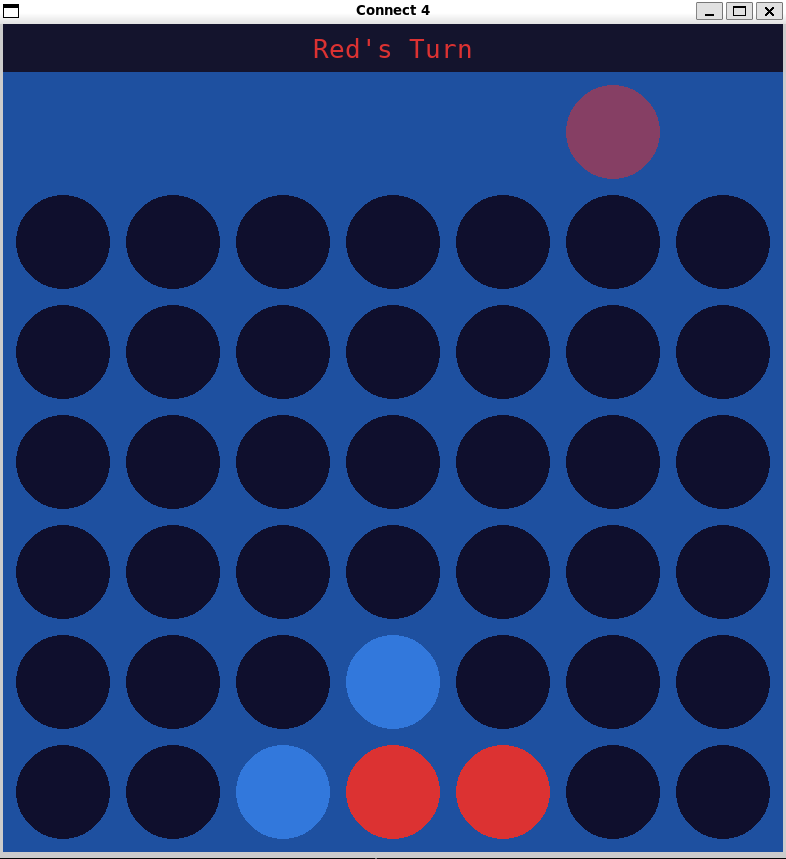
\includegraphics[width=0.3\linewidth]{Connect4AIPreLoseBlock}
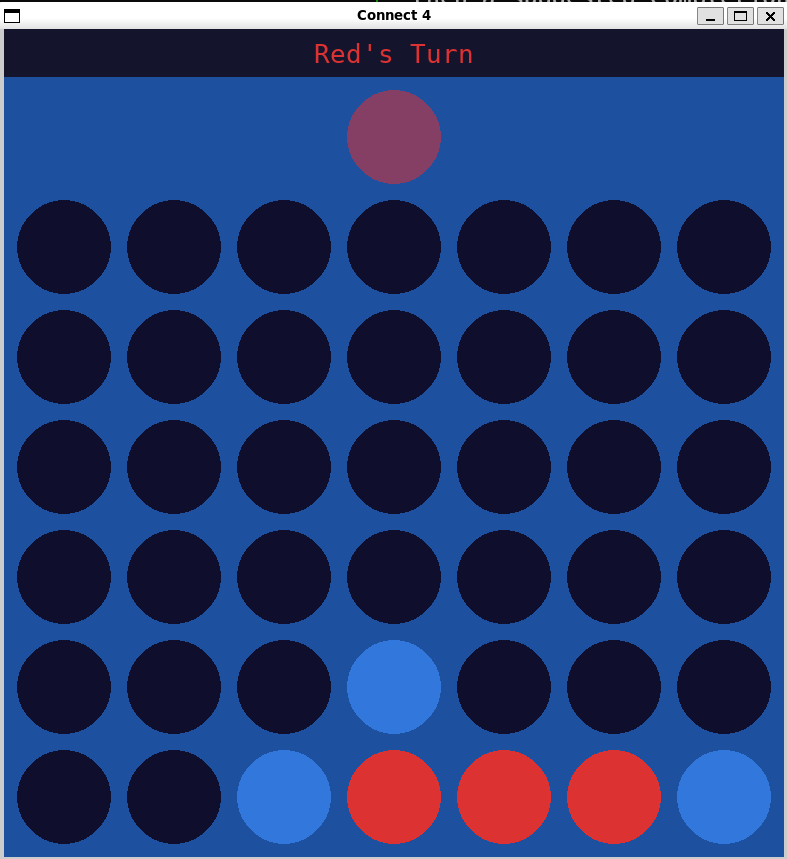
\includegraphics[width=0.3\linewidth]{Connect4AIPostLoseBlock}
    \caption{Before and after the AI (Blue) is able to block the Human (Red) win}
\label{fig:Blocking Loses}
\end{figure}

\begin{figure}[H]
\centering
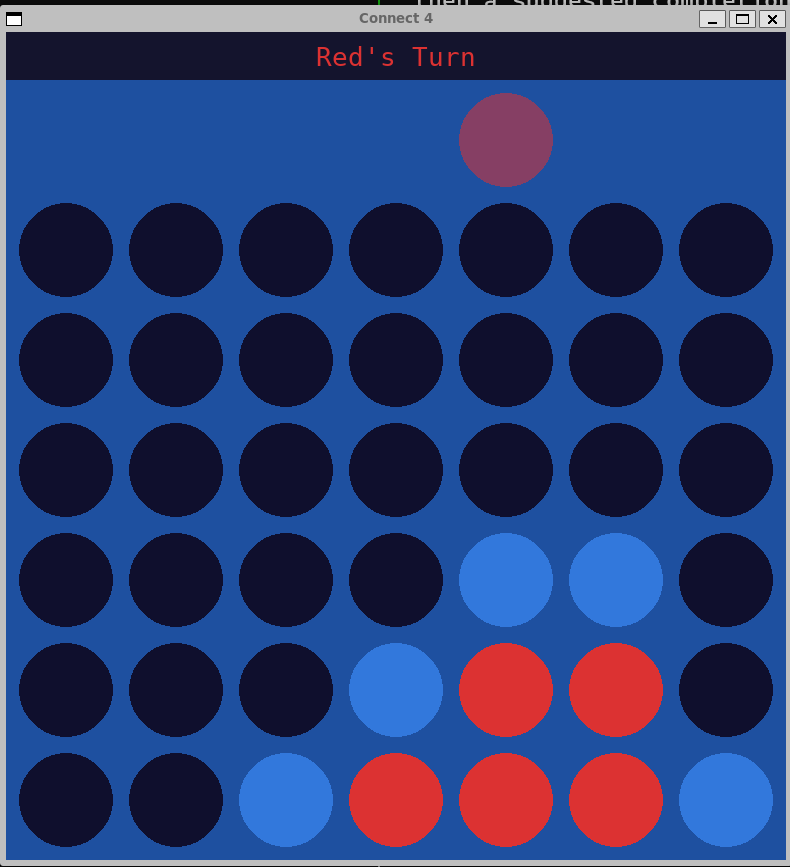
\includegraphics[width=0.3\linewidth]{Connect4AIPreWinTake}
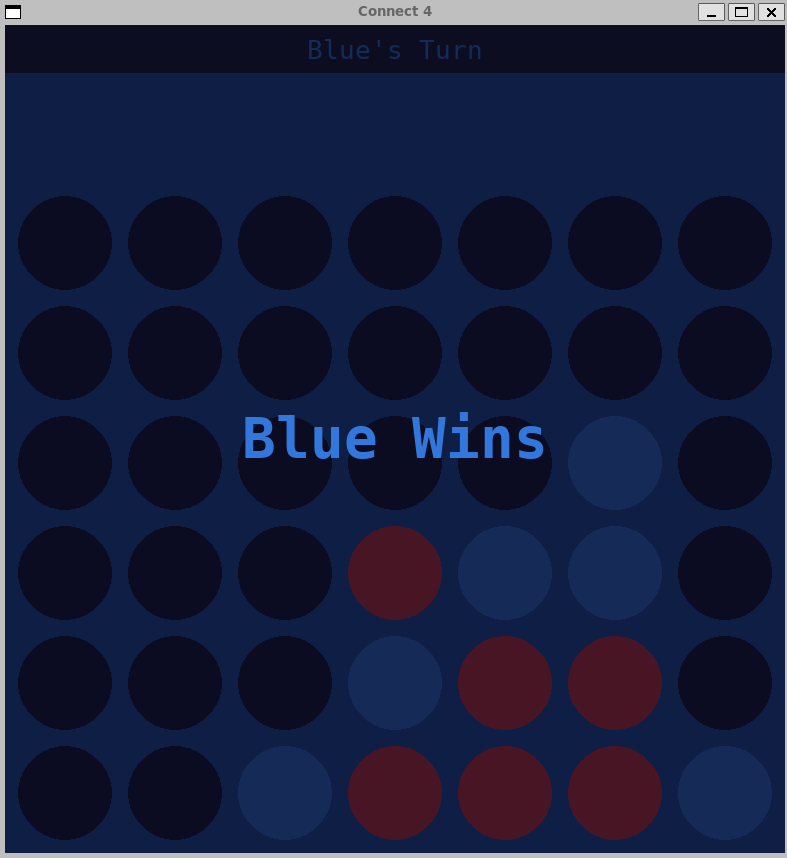
\includegraphics[width=0.3\linewidth]{Connect4AIPostWinTake}
\caption{Before and after the AI (Blue) correct plays the winning move}
\label{fig:Taking Wins}
\end{figure}

\begin{figure}[H]
\centering
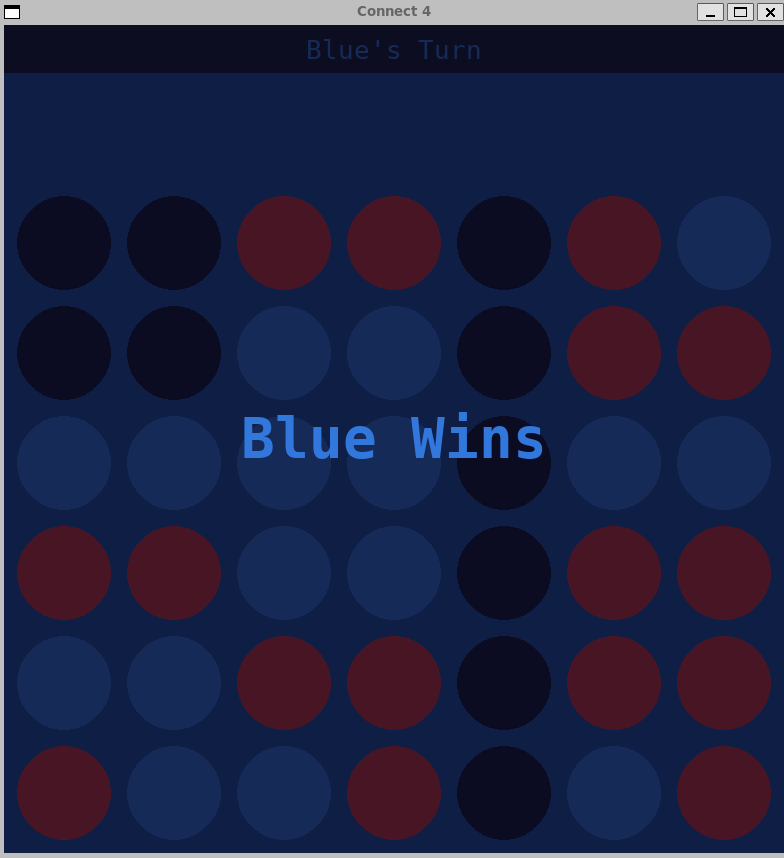
\includegraphics[width=0.3\linewidth]{Connect4AIvsAISelectiveDeepeningWithout}
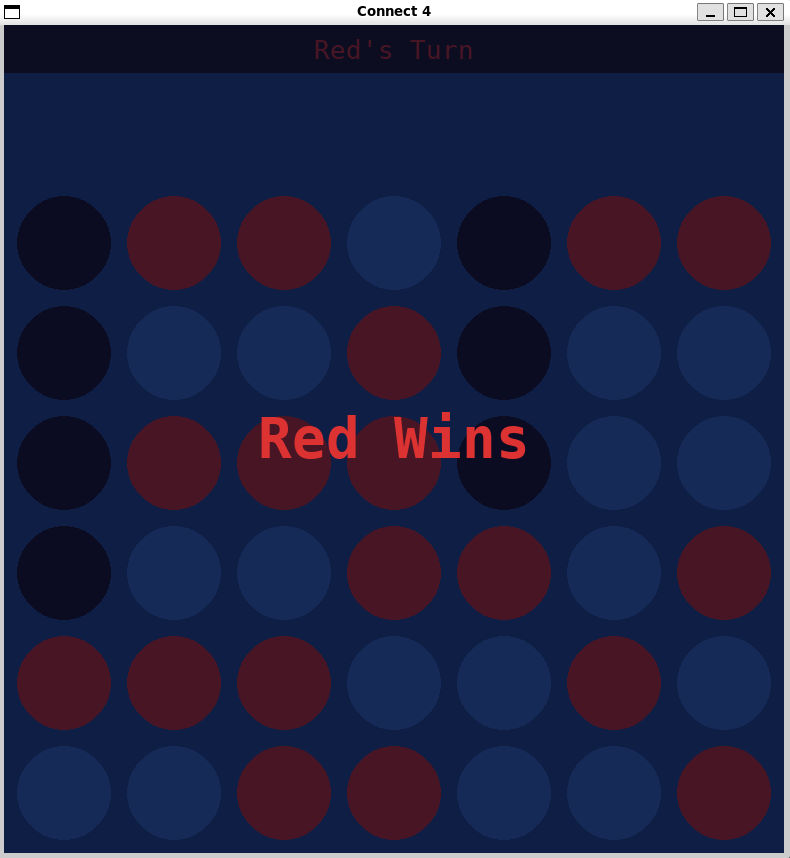
\includegraphics[width=0.3\linewidth]{Connect4AIvsAISelectiveDeepeningWith}
\caption{Game result AI vs AI depth 5, with and without Selective Deepening}
\label{fig:Selective Deepening Effect}
\end{figure}

% -------------------------------------------------------

\section*{Conclusion}

\end{document}
